% diagram_architecture_lora.png
% Two views side by side: the flow model as a stack of layer groups (left)
% and the LoRA adapter on one weight matrix (right).
% Canvas: 15.2303 cm x 5.00 cm (= \textwidth of the deck, height <= 5.0 cm).
\documentclass[border=0pt,11pt]{standalone}
\usepackage[T1]{fontenc}
\usepackage{lmodern}
\renewcommand{\familydefault}{\sfdefault}
\usepackage{amsmath}
\usepackage{tikz}
\usetikzlibrary{positioning,arrows.meta}

\definecolor{primaryNavy}{RGB}{24,24,27}
\definecolor{secondaryNavy}{RGB}{63,63,70}
\definecolor{mutedGray}{RGB}{248,250,252}
\definecolor{ruleGray}{RGB}{226,232,240}

\tikzset{
  box/.style={draw=secondaryNavy, line width=0.6pt, fill=mutedGray, rectangle,
              inner xsep=4pt, inner ysep=2.5pt, align=center,
              text=primaryNavy, font=\small},
  ar/.style={draw=secondaryNavy, line width=0.6pt,
             -{Latex[length=1.4mm,width=1.0mm]}},
  ln/.style={draw=secondaryNavy, line width=0.6pt},
  dline/.style={draw=secondaryNavy, line width=0.6pt, dashed},
  din/.style={draw=secondaryNavy, line width=0.6pt, dashed,
              -{Latex[length=1.4mm,width=1.0mm]}},
  alab/.style={text=primaryNavy, font=\small, align=center},
  note/.style={text=primaryNavy, font=\footnotesize, align=center},
}

\begin{document}
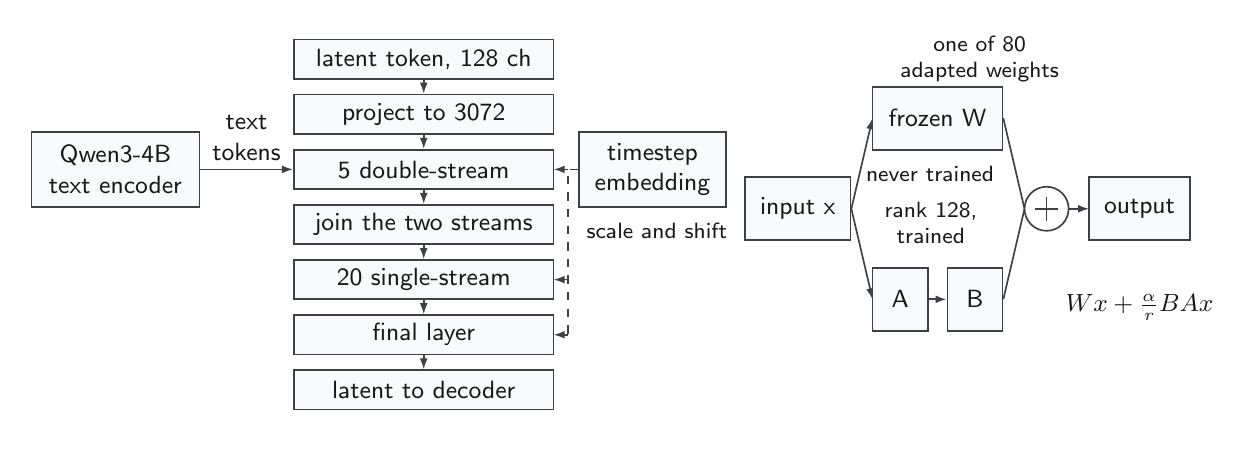
\begin{tikzpicture}[x=1cm,y=1cm]
\useasboundingbox (0,0) rectangle (15.2303,5.00);
\fill[white] (0,0) rectangle (15.2303,5.00);

% ================= LEFT PART: flow model stack, x = 0.05 .. 8.79 ===============
% rows of the stack (top to bottom), box x = 3.38 .. 6.68
\node[box, minimum width=3.30cm, minimum height=0.50cm] (s1) at (5.03,4.60) {latent token, 128 ch};
\node[box, minimum width=3.30cm, minimum height=0.50cm] (s2) at (5.03,3.90) {project to 3072};
\node[box, minimum width=3.30cm, minimum height=0.50cm] (s3) at (5.03,3.20) {5 double-stream};
\node[box, minimum width=3.30cm, minimum height=0.50cm] (s4) at (5.03,2.50) {join the two streams};
\node[box, minimum width=3.30cm, minimum height=0.50cm] (s5) at (5.03,1.80) {20 single-stream};
\node[box, minimum width=3.30cm, minimum height=0.50cm] (s6) at (5.03,1.10) {final layer};
\node[box, minimum width=3.30cm, minimum height=0.50cm] (s7) at (5.03,0.40) {latent to decoder};

\draw[ar] (s1.south) -- (s2.north);
\draw[ar] (s2.south) -- (s3.north);
\draw[ar] (s3.south) -- (s4.north);
\draw[ar] (s4.south) -- (s5.north);
\draw[ar] (s5.south) -- (s6.north);
\draw[ar] (s6.south) -- (s7.north);

% text encoder input (left of the stack)
\node[box, minimum width=2.13cm, minimum height=0.95cm] (enc) at (1.115,3.20) {Qwen3-4B\\text encoder};
\draw[ar] (enc.east) -- (s3.west);
\node[alab] at (2.78,3.60) {text\\tokens};

% timestep input (right of the stack); one branched dashed path into the stack
\node[box, minimum width=1.87cm, minimum height=0.95cm] (ts) at (7.935,3.20) {timestep\\embedding};
\draw[dline] (ts.west) -- (6.86,3.20) -- (6.86,1.10);
\draw[din] (6.86,3.20) -- (6.68,3.20);
\draw[din] (6.86,1.80) -- (6.68,1.80);
\draw[din] (6.86,1.10) -- (6.68,1.10);
\node[note] at (7.99,2.42) {scale and shift};

% ================= RIGHT PART: LoRA injection zoom, x = 9.05 .. 15.13 =================
% the zoom shows one of the adapted weights
\node[note] at (12.09,4.60) {one of 80\\adapted weights};

% input and fan out to the two branches
\node[box, minimum width=1.34cm, minimum height=0.80cm] (x) at (9.78,2.70) {input x};
\draw[ar] (x.east) -- (10.73,3.85);
\draw[ar] (x.east) -- (10.73,1.55);

% upper branch: frozen weight
\node[box, minimum width=1.65cm, minimum height=0.80cm] (fw) at (11.555,3.85) {frozen W};
\node[note] at (11.46,3.14) {never trained};

% lower branch: trained pair A, B
\node[box, minimum width=0.70cm, minimum height=0.80cm] (A) at (11.08,1.55) {A};
\node[box, minimum width=0.70cm, minimum height=0.80cm] (B) at (12.03,1.55) {B};
\draw[ar] (A.east) -- (B.west);
\node[note] at (11.47,2.52) {rank 128,\\trained};

% merge at the circled plus
\draw[ln] (fw.east) -- (12.66,2.70);
\draw[ln] (B.east)  -- (12.66,2.70);
\draw[ln, fill=white] (12.94,2.70) circle (0.28cm);
\draw[ln] (12.79,2.70) -- (13.09,2.70);
\draw[ln] (12.94,2.55) -- (12.94,2.85);

% output and formula
\draw[ar] (13.22,2.70) -- (13.48,2.70);
\node[box, minimum width=1.28cm, minimum height=0.80cm] (out) at (14.12,2.70) {output};
\node[text=primaryNavy, font=\small, align=center] at (14.12,1.45) {$Wx + \frac{\alpha}{r}BAx$};

\end{tikzpicture}
\end{document}
